%This section needs to be changed a lot
%Lets break it down into 'validation' and put that in the previous section
%
%I am adding another section which talks about the 'main' simulation

\section{Validation} %TODO: no longer a chapter

%small intro
In this section, we will discuss the simulation to validate our design and implementation. 
A scenario is created to validate that the updates from source nodes are delivered successfully when in range to the ferry node and the update packets are handled properly by the ferry node as designed.   
Further detail will be explained in the following subsequent section \ref{sec:scenario1}. %might remove this line


%When simulating each scenario, the following metrics will be measured:
%\begin{enumerate}
%	\item Time to update state in central repository (delay)
%	\item Variation in time to update state (delay jitter)
%	\item Number of state updates lost. Roughly corresponds to packet loss.
%	\item Memory utilization and packet dropping threshold within ferries.
%\end{enumerate}

%_________________________________________________________________
%________________________SCENARIO 1_______________________________
\subsection{Scenario Topology  and Details}
\label{sec:scenario1}


In Figure \ref{fig:scenario1}, it shows the topology to test if the gateway receives the update packets sent by the source nodes and if the ferry is picking up these update packets from source nodes when it moves past them.
There is one gateway node, one ferry node, and seven source nodes. 
The size of this topology is 0.75km x 0.75km with source nodes placed evenly apart by 0.375km. 
The gateway node is on the top left corner, and the ferry is in motion indicated next to a red arrow.
The speed of the ferry is a constant 60kph, as it moves clockwise two times along the rectangular path that is highlighted in white.  The simulated time is six minutes.

%picture of the rectangular path
\begin{figure}[ht]
    \centering
    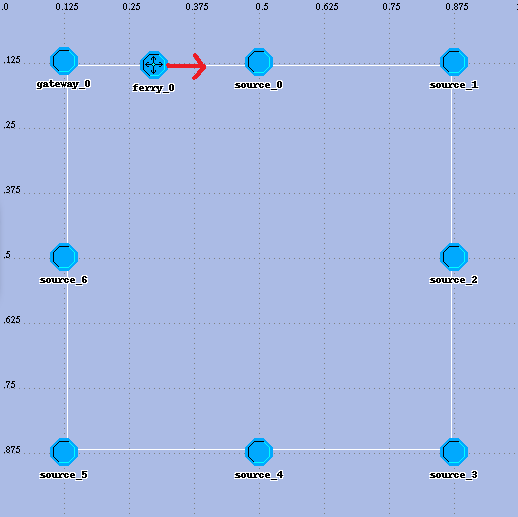
\includegraphics[width=.5\textwidth]{images/scenario1-top1r}
    \caption{Validation scenario topology}
    \label{fig:scenario1}
\end{figure}

\subsection{Validation Simulation Results}
\label{sec:results-validate}


After setting up OPNET to capture the desired statistics, the design and implementation are simulated.  The results are collected and shown in Figure \ref{fig:result1-a}.  From it, we can see that the ferry is picking up three update packets each time it passes by a source node.  This validates that ......

%result1-a   ferry receives update packets
\begin{figure}[ht]
    \centering
    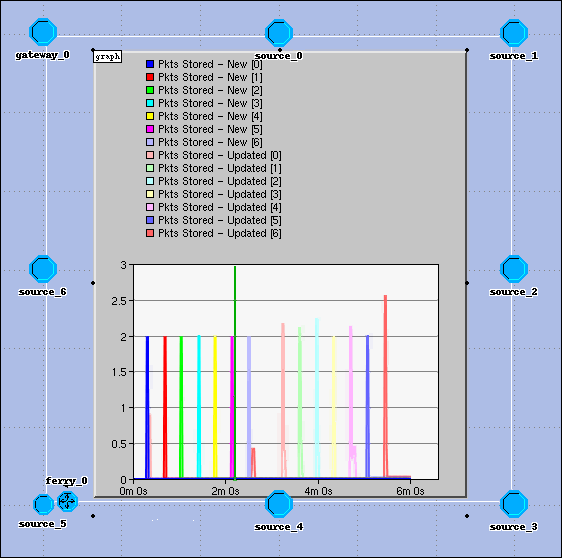
\includegraphics[width=.5\textwidth]{images/scenario1-result-received}
    \caption{Update packets received by the fery node}
    \label{fig:result1-a}
\end{figure}

The second part of the results is to see the if the gateway receives the update packets collected by the ferry node.  From Figure \ref{fig:result1-b}, there are two spikes in the graph which corresponds to the task of dumping the packets to the gateway node.  
The ferry node goes around two times for this simulation and that is why we see we two spikes.  
Each source node sends three update packets to the ferry node as it passes.  
Since there are seven source nodes, this accounts for the 20 packets received by the gateway node, which can be seen in Figure \ref{fig:result1-b}.


%result1-b   ferry delivers update packets to gateway
\begin{figure}[ht]
    \centering
    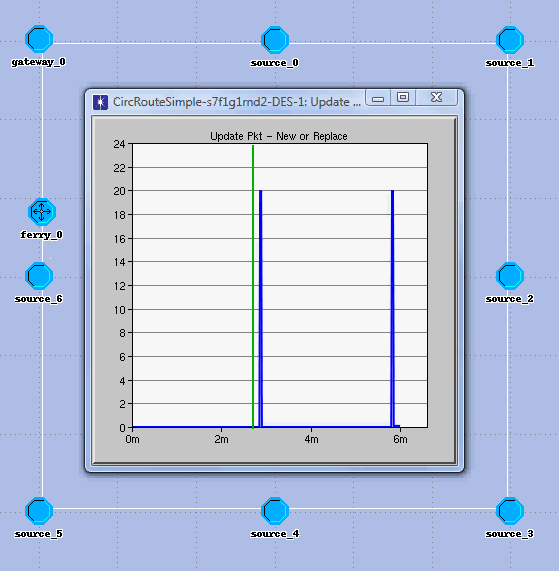
\includegraphics[width=.5\textwidth]{images/scenario1-result-gateway}
    \caption{Gateway receives the packet as the ferry node passes by its range of transmission}
    \label{fig:result1-b}
\end{figure}

